\documentclass[unicode, notheorems]{beamer}

\mode<presentation>
{
	\usetheme[numbers, totalnumbers, minimal]{Statmod}
	\setbeamercovered{transparent}
	\setbeamertemplate{caption}[numbered]
	\setbeamertemplate{enumerate item}[default]
	\setbeamertemplate{itemize item}[circle]
}

\usepackage[T2A]{fontenc}
\usepackage[utf8]{inputenc}
\usepackage[russian]{babel}
\usepackage{amsthm}
\usepackage{graphicx}
\usepackage{float}
\usepackage{subfig}
\usepackage{bm}

\DeclareMathOperator{\E}{\mathbb{E}}
\DeclareMathOperator{\Prb}{\mathbb{P}}
\DeclareMathOperator*{\argmax}{arg\,max\ }

\setbeamertemplate{navigation symbols}{}

\title[Оценивание расстояния на графах де Брёйна]{Задачи оценивания геномного расстояния на графах де Брёйна}

\author[Константинов А. В., гр. 15.Б04-мм]{Константинов Антон Владимирович, гр. 15.Б04-мм}
\institute[СПбГУ]{
	\small
	Санкт-Петербургский государственный университет \\
	Прикладная математика и информатика \\
	Вычислительная стохастика и статистические модели \\
	\vspace{0.4cm}
	Научный руководитель: к.ф.-м.н., доцент Коробейников~А. И. \\
	Рецензент: м.н.с. Шлемов~А. Ю.
	\vspace{0.3cm}
}
\date{
	Санкт-Петербург\\
	2019
}

\begin{document}

\begin{frame}
	\titlepage
\end{frame}

\begin{frame}{Задача сборки генома}
	\begin{block}{Основные термины}
	\begin{itemize}
		\item \textbf{Геномом} будем называть строку $\mathcal{S}$ над четырёхбуквенным алфавитом $\{A, T, G, C\}$.
		\item \textbf{Рид} (или \textbf{прочтение}) --- короткая подстрока $\mathcal{S}$.
		\item \textbf{$k$-мер} --- подстрока $\mathcal{S}$, имеющая длину $k$.
	\end{itemize}
\end{block}
\medskip
Пусть $\mathfrak{R}$ --- набор ридов для генома $\mathcal{S}$.\\
\medskip
\textbf{\color{blue} Задача сборки генома} \\
\smallskip
По набору строк $\mathfrak{R}$ восстановить (<<собрать>>) как можно более длинные \textbf{контиги} --- непрерывные подстроки исходной строки $\mathcal{S}$. В идеале хочется получить всю строку $\mathcal{S}$ целиком.
\end{frame}

\begin{frame}{Граф де Брёйна}
	Пусть $k$ --- положительное целое число.\\
	\bigskip
	\textbf{Сжатый граф де Брёйна строки $\mathcal{S}$} --- направленный мультиграф следующей конструкции:

	\begin{enumerate}
		\item Множество вершин графа --- множество всех $k$-меров строки $\mathcal{S}$.
		\item Для каждого $(k+1)$-мера, содержащегося в $\mathcal{S}$, в граф добавляется ребро $v_1 \to v_2$, где $v_1$ и $v_2$ --- его префикс и суффикс длины $k$ соответственно. Кратность такого ребра равна количеству вхождений соответствующего $(k+1)$-мера в геном.
		\item Пути, не имеющие разветвлений, заменяются рёбрами путём конкатенации соответствующих $(k+1)$-меров.
	\end{enumerate}
\end{frame}

\begin{frame}{Проблема повторов}
\begin{block}{Геномный путь}
	В графе де Брёйна строки $\mathcal{S}$ \textit{существует} соответствующий исходной строке $\mathcal{S}$ \textit{эйлеров путь}, то есть путь, проходящий по каждому ребру мультиграфа ровно столько раз, какова его кратность. Будем называть этот путь \textbf{геномным}.
\end{block}

\textbf{Проблема}: повторы последовательностей (длины больше $k$).\\
\bigskip
\begin{minipage}{0.55\textwidth}
	\includegraphics[width=0.9\textwidth]{img/repeat-resolution-good}
\end{minipage}%
\begin{minipage}{0.45\textwidth}
	Пусть $\mathcal{S} = \mathbf{e_1 f e_2 \ldots g_1 f g_2}$, где $\mathbf{e}_i$, $\mathbf{g}_i$ и $\mathbf{f}$ --- некоторые строки.\\
	{\color{blue} Как должен проходить геномный путь?}
\end{minipage}\\
\bigskip
\textbf{Идея}:  будем сравнивать геномные и графовые расстояния между ридами.

\end{frame}

\begin{frame}{Постановка задачи}
	Зафиксируем пару $\mathbf{e}_1, \mathbf{e}_2$ рёбер графа де Брёйна. Будем предполагать, что
	\begin{enumerate}
		\item  $\mathbf{e}_1 = \mathcal{S}[a, b]$ и $\mathbf{e}_2 = \mathcal{S}[c, d]$, где $a < c$;
		\item $\mathbf{e}_1$ и $\mathbf{e}_2$ соединяет путь $\bm p =  \mathbf{e}_1 \to p_1 \to \ldots \to p_m \to \mathbf{e}_2$.
	\end{enumerate}
	\bigskip
	{\bf Графовое расстояние:} $d_{\mathrm{graph}} (\mathbf{e}_1, \mathbf{e}_2; \bm p) = \sum_{i=1}^m |p_i| - (m+1)k$,\\
	\medskip
 	{\bf Геномное расстояние:} $d_{\mathrm{genome}}(\mathbf{e}_1, \mathbf{e}_2) = c - b$.\\
 	\bigskip
	Определим множества
	\begin{gather*}
		\mathbf{D}_{\mathrm{graph}} = \big\{ d_{\mathrm{graph}} (\mathbf{e}_1, \mathbf{e}_2; \bm p)\  |\  \bm p \text{ --- путь, соединяющий } \mathbf{e}_1 \text{ с } \mathbf{e}_2  \big\} , \\
		\mathbf{D}_{\mathrm{genome}} = \big\{  d_{\mathrm{genome}}(\mathbf{e}_1^{(i)}, \mathbf{e}_2^{(j)})\ \mid \mathbf{e}_s^{(t)} \text{ --- } t \text{-ое вхождение } \mathbf{e}_s \text{ в геном } \mathcal{S} \big\},
	\end{gather*}\\ 
	\textsc{ \large \color{blue} Задача:}
	Найти пересечение $\mathbf{D} = \mathbf{D}_{\mathrm{graph}} \cap \mathbf{D}_{\mathrm{genome}}$.
	\end{frame}

\begin{frame}{Вероятностная модель парных ридов}

{\color{blue} \bf Из чего состоит библиотека ридов $\mathfrak{R}$?}\\
\medskip
Пусть
\begin{enumerate}
	\item  $\xi$ --- дискретная случайная величина с носителем $\{ 1, \ldots, |\mathcal{S}|\}$, имеющая смысл координаты в геноме,
	\item $\eta$ --- независимая от $\xi$ неотрицательная целочисленная случайная величина (т. н. \textbf{длина вставки}),
	\item $\ell$ --- положительное целое число (\textbf{длина рида}).
\end{enumerate}
\begin{block}{}
	\begin{enumerate}
		\item Фрагмент --- подстрока генома, имеющая вид $\mathcal{S}[\xi, \xi+\eta]$;
		\item Левый рид --- префикс длины $\ell$ фрагмента, т. е. подстрока  $\mathcal{S}[\xi, \xi+\ell]$;
		\item Правый рид --- суффикс длины $\ell$ фрагмента, т.е. подстрока $\mathcal{S}[\xi+\eta-\ell, \xi+\eta]$.
	\end{enumerate}
\end{block}
\end{frame}

\begin{frame}{Вероятностный подход к задаче}
	\begin{figure}	
		\centering
		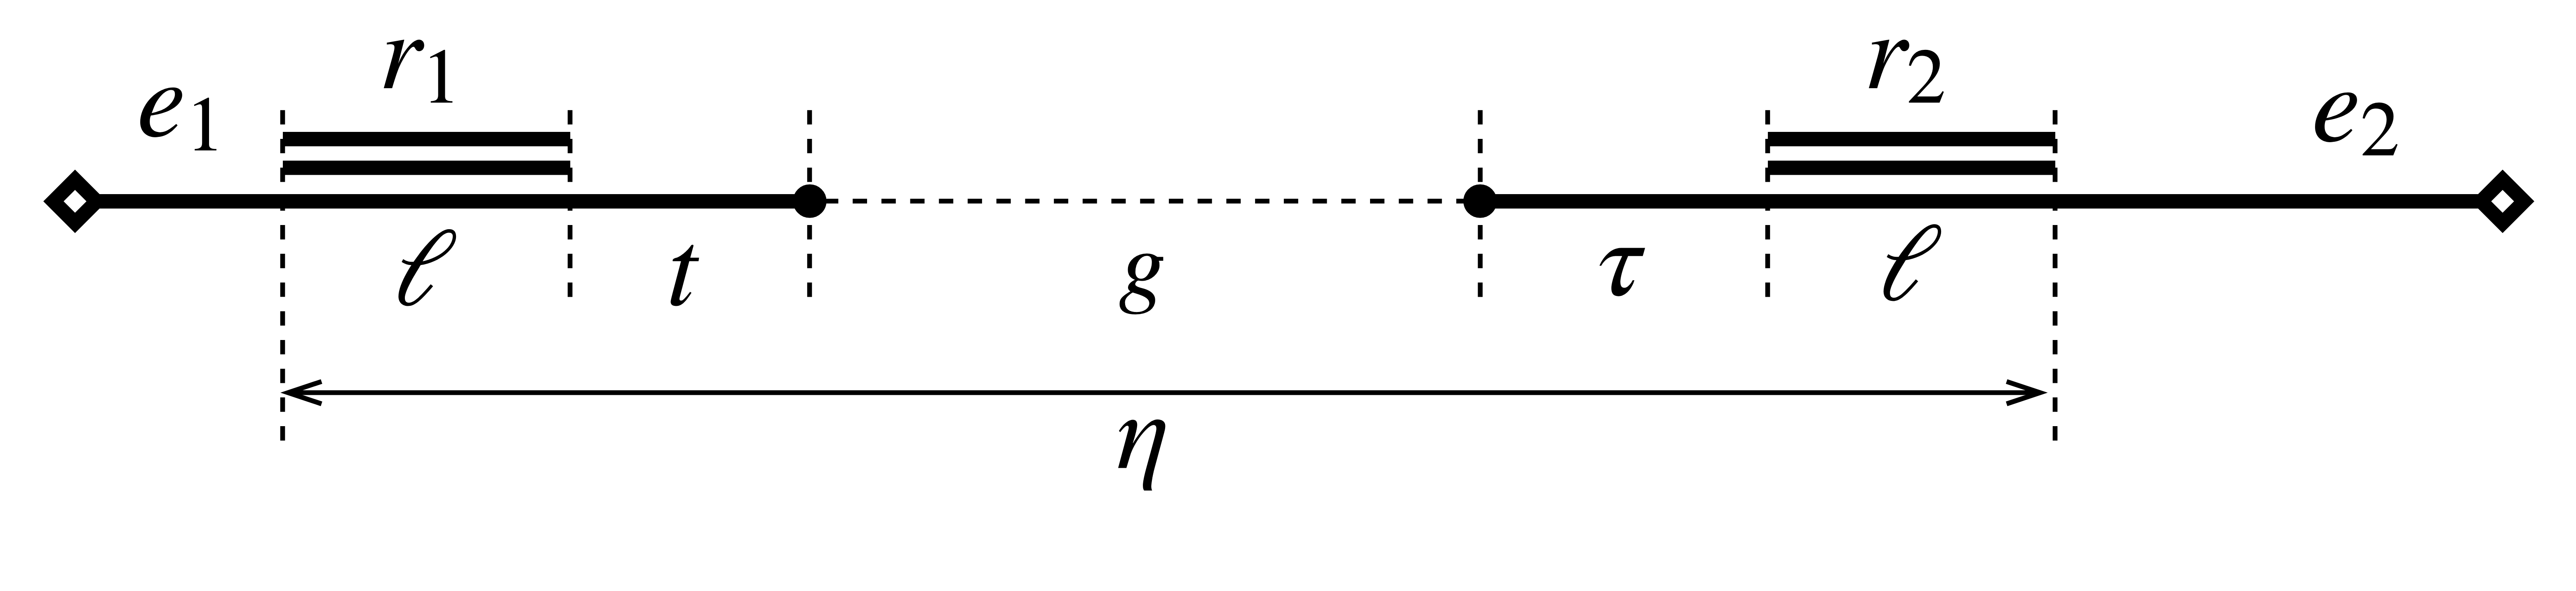
\includegraphics[scale=0.05]{img/alignment_shifted}
		\caption{Расположение ридов на рёбрах графа}
	\end{figure}

	Пусть $(r_1, r_2) \in \mathfrak{R}$, и $r_i$ является подстрокой ребра $\mathbf{e}_i$ ($i=1,2$). \\
	\medskip
	Введём обозначения: 
	\begin{enumerate}
		\item $g$ --- геномное расстояние между $\mathbf{e}_1$ и $\mathbf{e}_2$,
		\item $t$ --- расстояние от конца $r_1$ до конца $\mathbf{e}_1$,
		\item $\tau$ --- координата начала $r_2$ на $\mathbf{e}_2$.
	\end{enumerate}
\end{frame}

\begin{frame}{Вероятностный подход к задаче}
	Рассмотрим формально выборку $\Big( (t_1, \tau_1, g_1), \ldots, (t_n, \tau_n, g_n) \Big)$.
	\begin{enumerate}
		\item Реализации $(t, \tau)$ наблюдаются только при условии $A_{\mathbf{e}_2}(r_2) = \{\text{рид } r_2 \text{ приложен к } \mathbf{e}_2\}$ (будем считать, что $r_1$ уже приложен);
		\item Реализации $g$ не наблюдаются вовсе.
	\end{enumerate}
	\smallskip
	При этом
	\begin{enumerate}
		\item Совместное распределение вектора $(t_i, \tau_i)$ зависит от $g_i$ как от параметра.
		\item $t_i$, $\tau_i$ и $g_i$ связаны соотношением $\tau_i = \eta_i - t_i - g_i - 2\ell$, где $g_i  \in \mathbf{D}$.
	\end{enumerate}
	\smallskip
	Получаем набор реализаций $\mathbb{T} = \Big( (t_1, \tau_1), \ldots, (t_n, \tau_n) \Big)$.\\
	\medskip
	{\color{blue} В этом случае исходная задача сводится к статистическому выводу для $g_i$ по $\mathbb{T}$.}
\end{frame}

\begin{frame}{Апостериорное распределение для одной реализации}
Было получено выражение для функции вероятности $p(g \mid t, \tau, A_{\mathbf{e}_2})$.
\begin{block}{Предложение}
	Пусть длина вставки $\eta$ имеет распределение $\mathcal{P}_\eta$ с функцией распределения $F(x) = \Prb(\eta < x)$. Будем считать, что априорно $g$ равномерно распределена на $\mathbf{D}_{\mathrm{graph}}$.\\
	\medskip
	Тогда
	\begin{equation*}
	\begin{gathered}
	p(g \mid t, \tau,  A_{\mathbf{e}_2}) =  \frac{q(\tau, g, t)}{\sum_{j=1}^k q(\tau, g^{(j)}, t)}	\,,
	\end{gathered}
	\end{equation*}
	где
	\begin{equation*}
		q(x, y, z)  = \frac{F\big(x+y+z+2\ell+1\big) - F\big(x+y+z+2\ell\big)}{F( y + z + \ell + M) - F(y + z + 2\ell)}\,.
	\end{equation*}
\end{block}
\end{frame}

\begin{frame}{Переход к случаю нескольких реализаций}
	\begin{itemize}
		\item На практике для каждого рида  $(r_1, r_2) \in \mathfrak{R}$ реализуется собственное расстояние $g^{(i)} \in \mathbf{D}_{genome}$ для некоторого $i$.
		\item Поэтому нельзя напрямую сделать переход к повторной независимой выборке, как это обычно бывает в статистике.
	\end{itemize}
	\medskip
	Приходим к {\color{blue} модели смеси}:
	\begin{equation*}
		(t, \tau) \sim \sum_{i=1}^k \pi_i  \mathcal{L}_{\tau, t} \big(g^{(i)}\big), \text{ где } \pi_i \ge 0 \text{ и } \sum_{i=1}^k \pi_i = 1.
	\end{equation*}
	Здесь $\pi_i$ мы можем оценить, усредняя апостериорную вероятность $p(g^{(i)} \mid t, \tau, A_{\mathbf{e}_2})$ по всем имеющимся реализациям.
\end{frame}

\begin{frame}{Апостериорное распределение для $n$ реализаций}
	Получено следующее утверждение, дающее апостериорное распределение $g$ при условии набора реализаций $(t, \tau)$.
	\begin{block}{Предложение}
		Пусть длина вставки $\eta$ имеет распределение $\mathcal{P}_\eta$ с функцией распределения $F(x) = \Prb(\eta < x)$. Будем считать, что априорно $g$ равномерно распределена на $\mathbf{D}_{\mathrm{graph}}$.\\
		\medskip
		Тогда
		\begin{equation*}
		p(g \mid \mathbb{T}, A_{\mathbf{e}_2}) = \frac{1}{n} \sum_{i = 1}^n \left[ \frac{q(\tau_i, g, t_i)}{\sum_{j=1}^k q(\tau_i, g^{(j)}, t_i)} \right]\,,
		\end{equation*}
		где
		\begin{equation*}
			q(x, y, z)  = \frac{F\big(x+y+z+2\ell+1\big) - F\big(x+y+z+2\ell\big)}{F( y + z + \ell + M) - F(y + z + 2\ell)}\,.
		\end{equation*}
	\end{block}
\end{frame}

\begin{frame}{Данные}
	Во всех следующих примерах используются графы де Брёйна, построенные по различным библиотекам ридов для первых 400 тысяч нуклеотидов генома \textit{E.coli} (штамм \textit{K12 MG1655}).\\
	\medskip
	{\color{blue} Реальные риды.} Были рассмотрены две библиотеки:
	\begin{enumerate}
		\item Первая (<<Библиотека A>>) имеет близкое к нормальному распределение $\eta$. Использовалась ф. р. нормального распределения с оценёнными параметрами ($\mu \approx 215$, $\sigma \approx 10$).
		\item Для второй библиотеки (<<Библиотека Б>>) в качестве $F$ использовалась эмпирическая ф. р. ($\mathrm{med}\ \eta \approx 480$).
	\end{enumerate}
\end{frame}

\begin{frame}{Распределения длины вставки}
		\begin{figure}%
			\centering
			\subfloat[Библиотека А. Хорошо аппроксимируется нормальным с параметрами $\mu = 215$, $\sigma = 10$]{{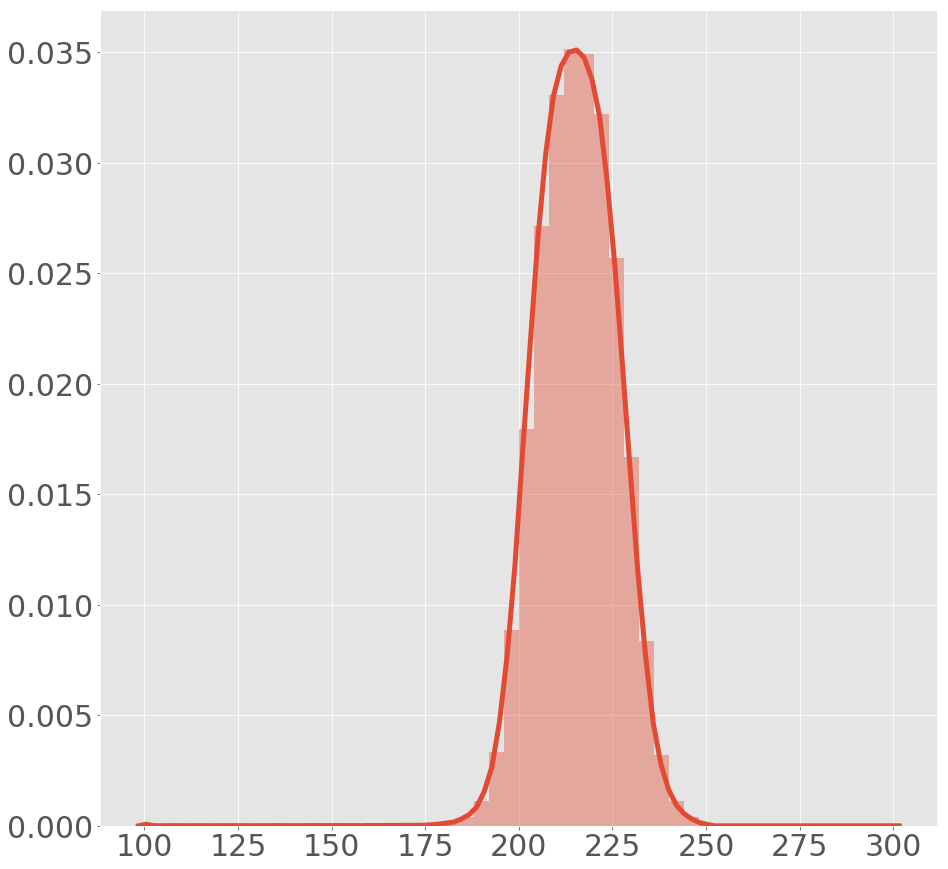
\includegraphics[width=0.45\linewidth]{fig/real-reads/good-lib/hist} }}%
			\qquad
			\subfloat[Библиотека Б. Используем эмпирическую ф. р.,  $\mathrm{mode}\ \eta = 480$]{{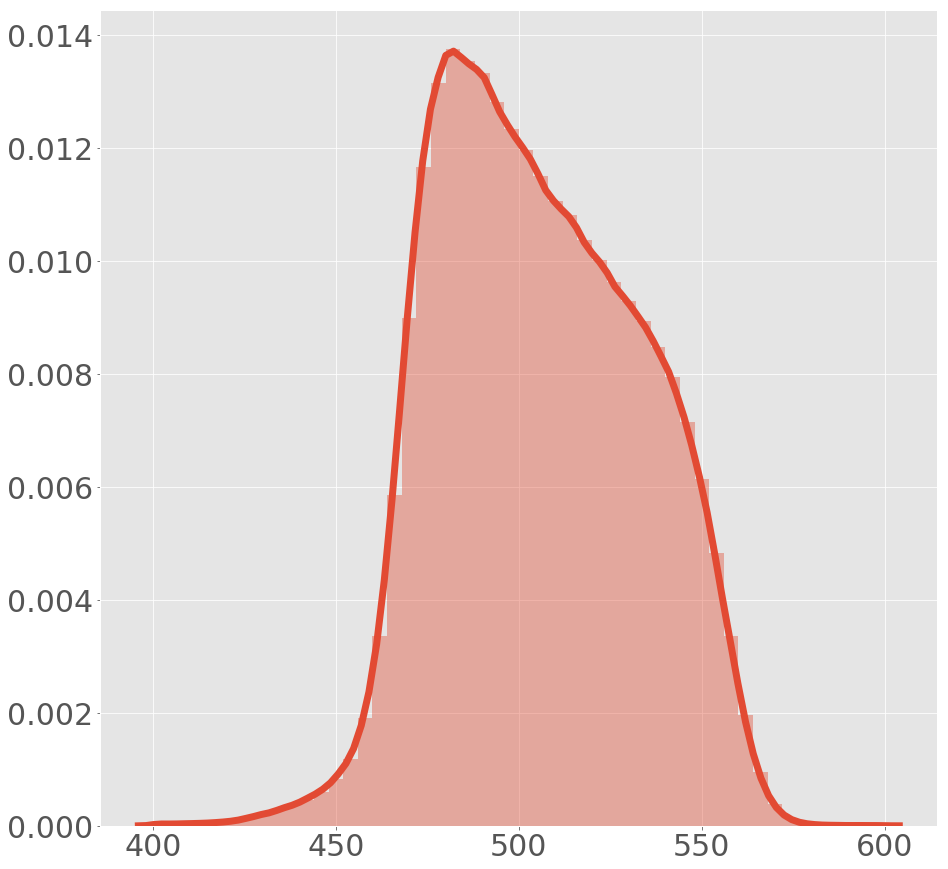
\includegraphics[width=0.45\linewidth]{fig/real-reads/bad-lib/hist} }}%
			\caption{Распределения длины вставки для библиотек А и Б}
		\end{figure}
\end{frame}

\begin{frame}{Библиотека А}
	\begin{figure}%
		\centering
		\subfloat[Апостериорное распределение]{{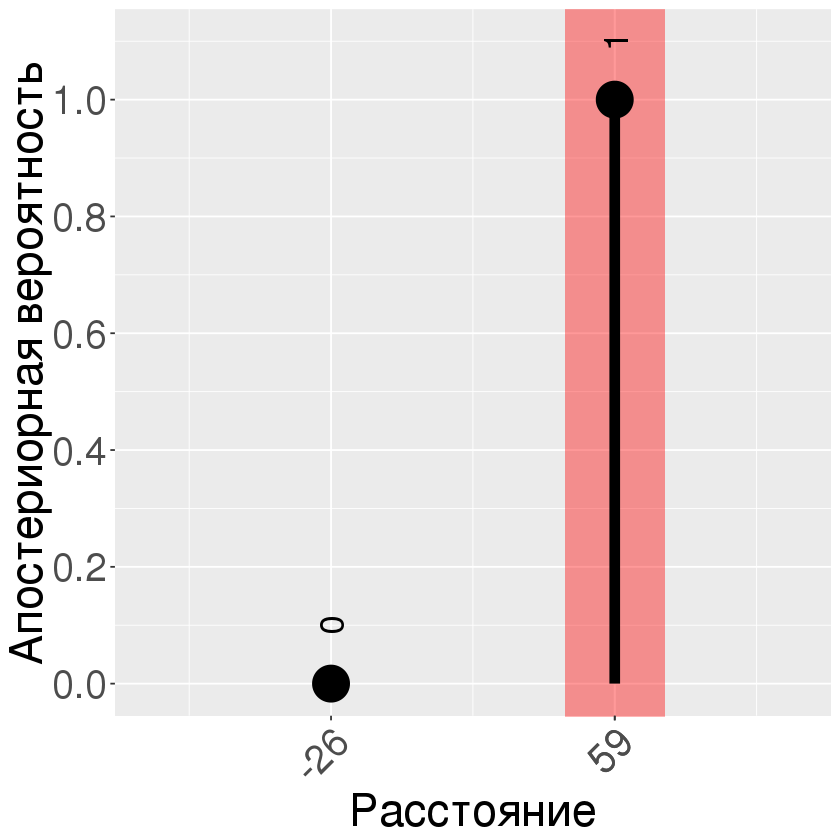
\includegraphics[width=0.45\linewidth]{fig/real-reads/good-lib/4-posterior} }}%
		\qquad
		\subfloat[Гистограмма $\eta - g$]{{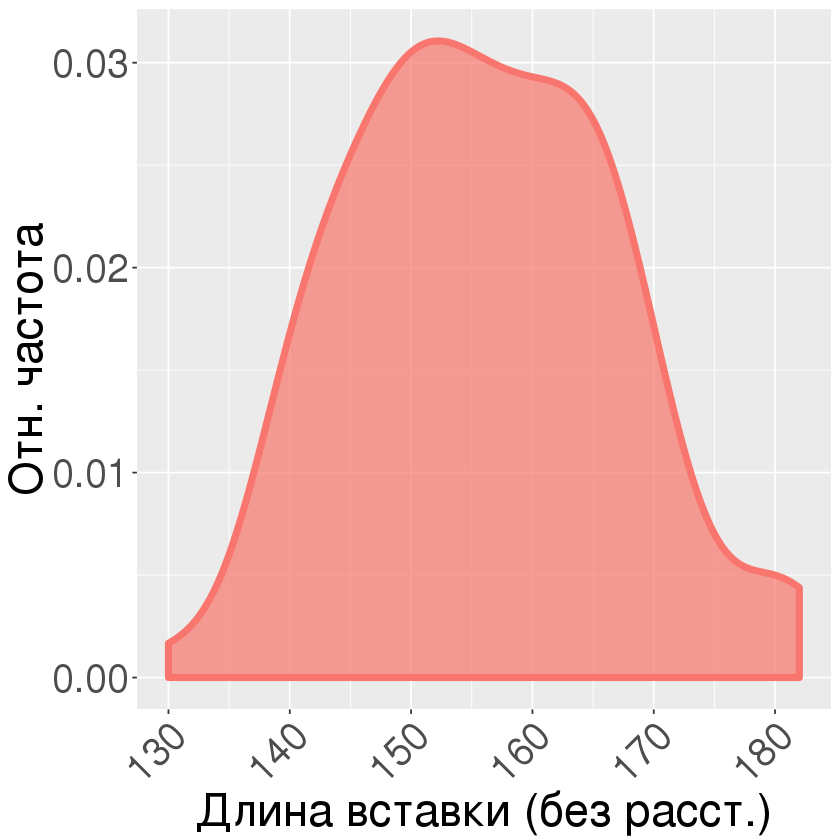
\includegraphics[width=0.45\linewidth]{fig/real-reads/good-lib/4-is} }}%
		\caption{Неповторные рёбра}
	\end{figure}
\end{frame}

\begin{frame}{Библиотека А}
	\begin{figure}%
		\centering
		\subfloat[Апостериорное распределение]{{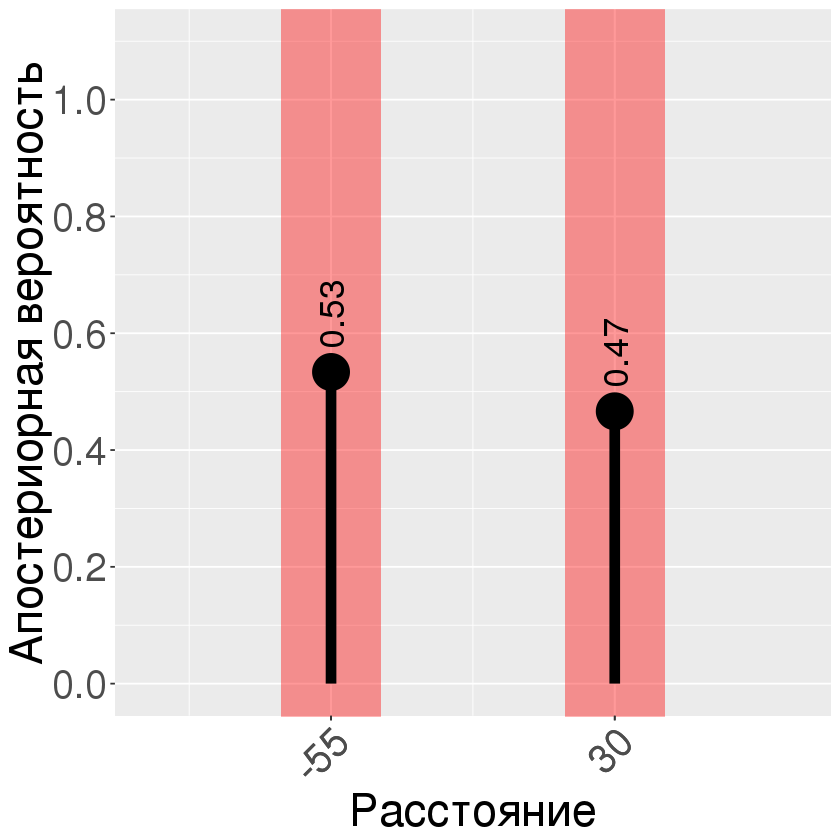
\includegraphics[width=0.45\linewidth]{fig/real-reads/good-lib/1-posterior} }}%
		\qquad
		\subfloat[Гистограмма $\eta - g$]{{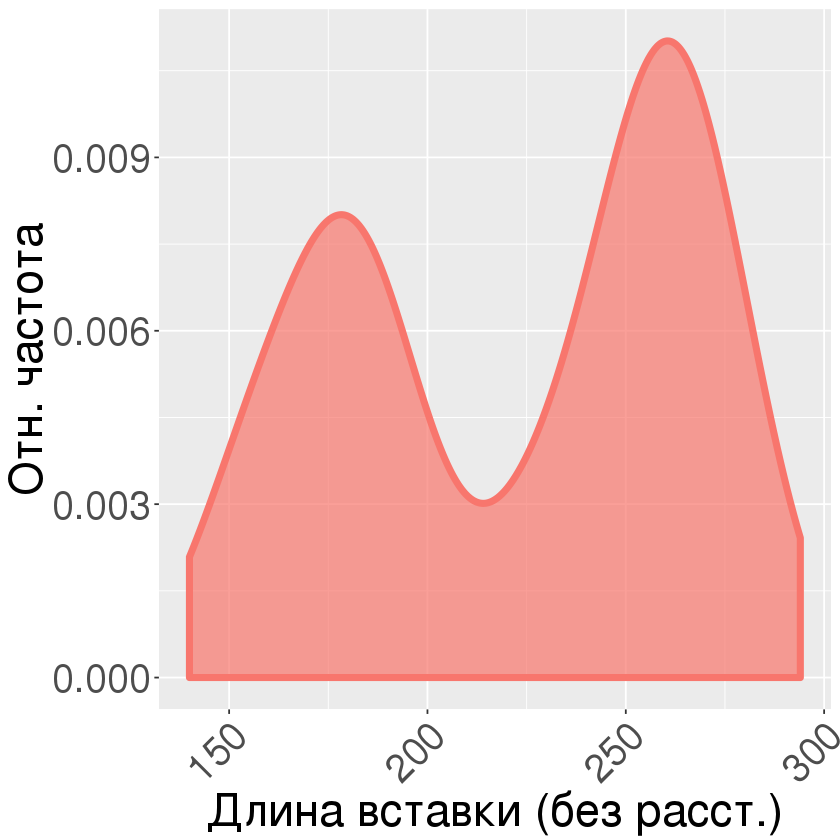
\includegraphics[width=0.45\linewidth]{fig/real-reads/good-lib/1-is} }}%
		\caption{Одно из рёбер имеет двойную кратность}
	\end{figure}
\end{frame}

\begin{frame}{Библиотека Б}
\begin{figure}%
	\centering
	\subfloat[Апостериорное распределение]{{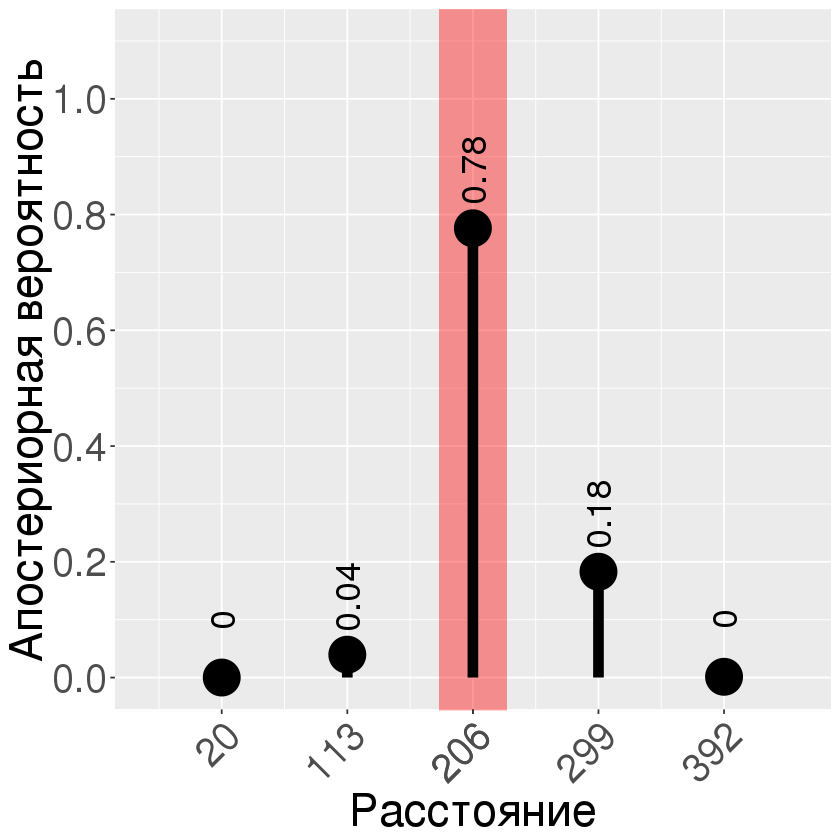
\includegraphics[width=0.45\linewidth]{fig/real-reads/bad-lib/4-posterior} }}%
	\qquad
	\subfloat[Гистограмма $\eta - g$]{{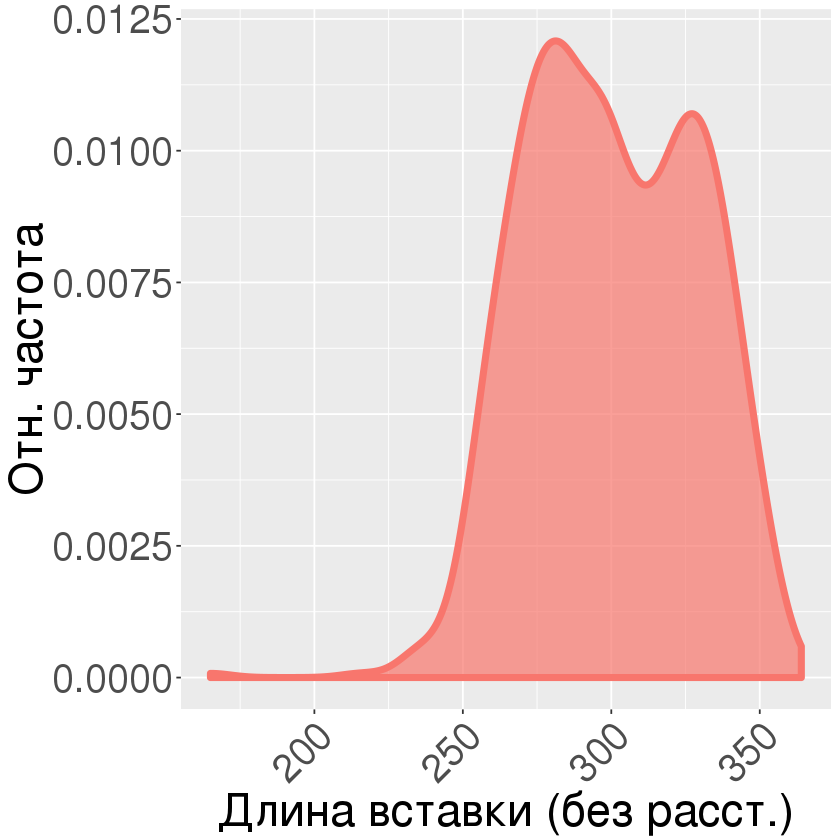
\includegraphics[width=0.45\linewidth]{fig/real-reads/bad-lib/4-is} }}%
	\caption{Неповторные рёбра}
\end{figure}
\end{frame}

\begin{frame}{Библиотека Б}
	\begin{figure}%
		\centering
		\subfloat[Апостериорное распределение]{{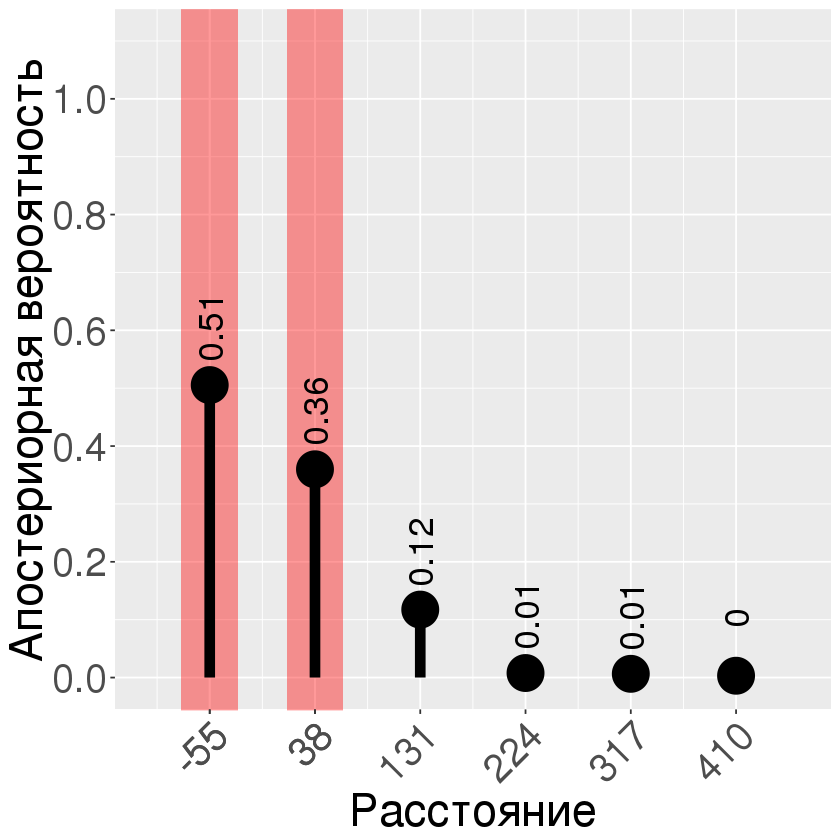
\includegraphics[width=0.45\linewidth]{fig/real-reads/bad-lib/2-posterior} }}%
		\qquad
		\subfloat[Гистограмма $\eta - g$]{{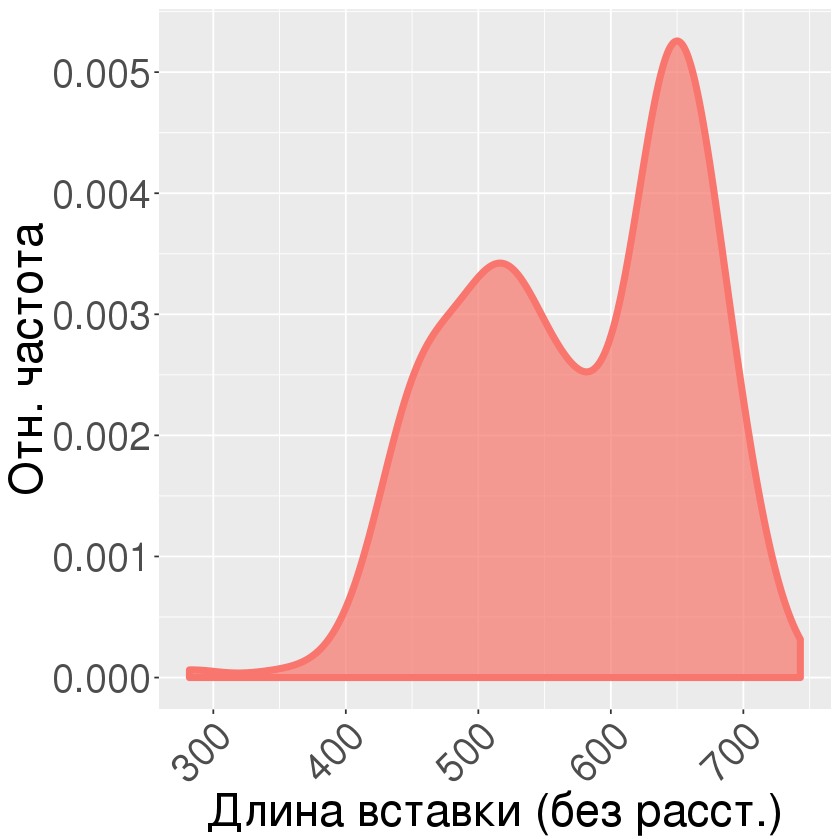
\includegraphics[width=0.45\linewidth]{fig/real-reads/bad-lib/2-is} }}%
		\caption{Одно из рёбер имеет двойную кратность}
	\end{figure}
\end{frame}

\begin{frame}{Библиотека Б}
\begin{figure}%
	\centering
	\subfloat[Апостериорное распределение]{{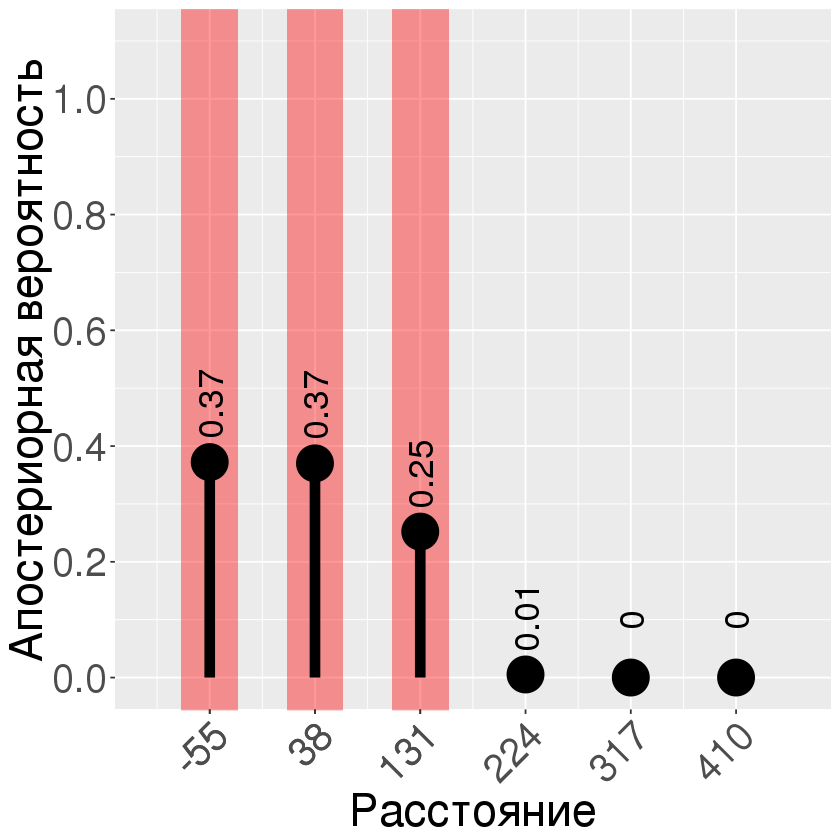
\includegraphics[width=0.45\linewidth]{fig/real-reads/bad-lib/3-posterior} }}%
	\qquad
	\subfloat[Гистограмма $\eta - g$]{{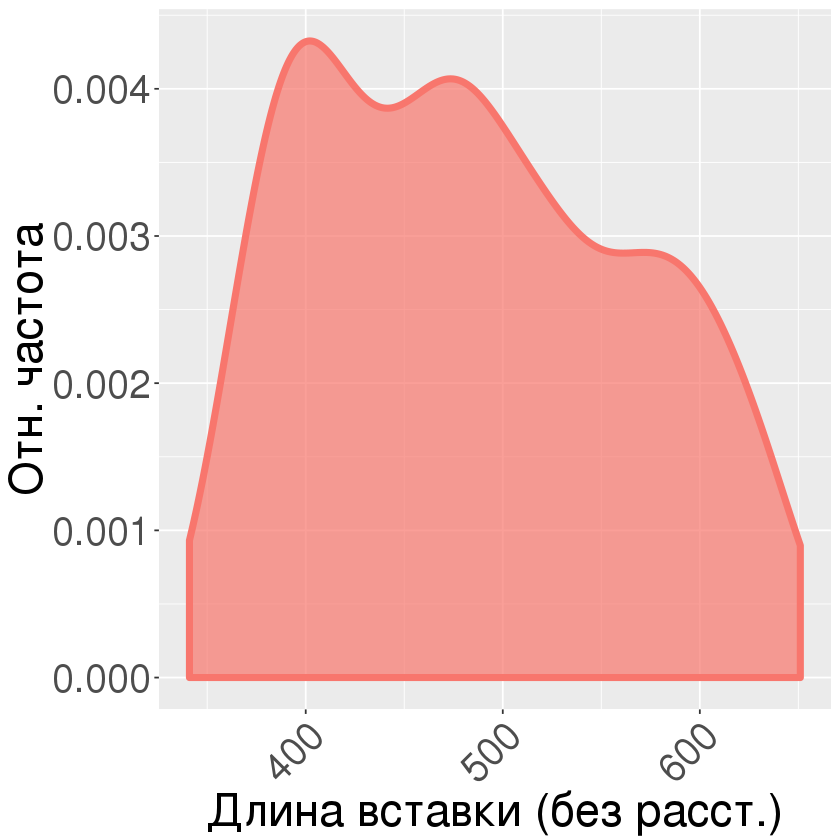
\includegraphics[width=0.45\linewidth]{fig/real-reads/bad-lib/3-is} }}%
	\caption{Одно из рёбер имеет тройную кратность}
\end{figure}
\end{frame}

\begin{frame}{Заключение}
	В работе была рассмотрена задача оценки геномных расстояний между рёбрами в графе де Брёйна.
	\bigskip
	\begin{enumerate}
		\item Построена вероятностная модель, позволяющая получать требуемые оценки в виде апостериорных вероятностей для расстояний, имеющихся в графе.
		\item Построенная модель протестирована на реальных геномных данных.
	\end{enumerate}
	\bigskip
	В дальнейшем полученные оценки, например, могут быть применены в геномных ассемблерах для разрешения повторов в графе де Брёйна. 
\end{frame}

\end{document}
